\section*{Preprint Framing Draft}

\subsection*{Working Title}
\textbf{Meta-Stable Architectures, Volume V: Adaptive RC as an Instructor Model in Heterogeneous Networks}

\subsection*{Abstract}
We extend the fixed Reflective Coordinator (RC) of Volume IV into an adaptive instructor-like coordination layer for heterogeneous networks. The proposed model reads group state through phase dispersion, lag, local error proxies, anchor structure, and bounded episode memory, then adjusts coordination in a soft-control regime without enforcing rigid synchrony. We test lesson-like protocols with distinct disturbance types, including noise-, lag-, and contagion-dominated episodes, and compare repeated sessions under heterogeneous agent populations. The clearest current result is not a dramatic gain in coarse recovery-time metrics, but a consistent reduction in field error once mutual attunement between coordinator and group is introduced. This suggests that adaptive coordination may first improve field quality and reduce turbulence before yielding strong gains in headline recovery observables. Group memory remains a plausible bounded extension, but its long-horizon role is still under investigation.

\subsection*{Introduction Draft}
Volume V is best understood as a disciplined continuation of Volume IV. Volume IV introduced the Reflective Coordinator as a bounded soft coordination layer capable of restoring recovery in networked metastable systems without hard control. The next natural question is whether such a coordinator can remain soft while becoming more responsive to the actual state of a heterogeneous group.

The present volume answers this question by reinterpreting Adaptive RC as an Instructor Model. The key shift is conceptual: the coordinator is no longer treated as a fixed metronome, but as a state-reading layer that observes how the group is responding. In practical terms, this means tracking not only phase dispersion, but also lag, local error proxies, anchor structure, and later, bounded traces of meaningful collective episodes.

This shift is motivated by a simple but important observation: heterogeneous groups do not fail in only one way. Some disturbances are predominantly noisy, some produce delayed response, and some spread locally through contagion-like destabilization. A useful coordinator therefore should not be judged only by a single mean recovery time. It should also be evaluated by whether it preserves recoverability under diversity, reduces local error, and prevents the field from becoming turbulent.

Our current simulations support this narrower and more defensible interpretation. The strongest present result is not yet a large gain in headline recovery metrics over earlier adaptive variants. Instead, the clearest effect appears when repeated lesson-like protocols are introduced and the group is allowed to become gradually attuned to the instructor signal. Under this mutual attunement, peak field error drops substantially across repeated sessions even when coarse recovery-time and tail metrics change only weakly. This suggests that adaptive coordination may first improve field quality before it improves global speed-like observables.

For this reason, Volume V should be read as an exploratory but coherent step: from fixed soft coordination toward instructor-like coordination in heterogeneous networks, with mutual attunement as the strongest current learning result and bounded group memory as an important but still secondary extension.

\subsection*{Results Framing}
At the current stage, the simulation results support four claims.
\begin{itemize}
    \item The fixed RC of Volume IV can be extended into a bounded state-aware coordination layer.
    \item Different lesson types, especially noise-, lag-, and contagion-dominated episodes, generate distinct field regimes and should not be collapsed into a single generic stress protocol.
    \item Mutual attunement between coordinator and group reduces field error across repeated lessons.
    \item Bounded group memory $K_g$ remains plausible as compressed episode memory, but is not yet the strongest practical result.
\end{itemize}

The simulations do \emph{not} yet justify stronger claims of large superiority in recovery-time metrics, nor a mature theory of long-horizon group learning. These remain future directions.

\subsection*{Suggested Figures}
The following figures are the most natural candidates for the current preprint framing.
\begin{itemize}
    \item State-aware / adaptive sanity figure:
    \texttt{manuscripts/v4/figures/adaptive\_rc\_first\_demo\_plot.png}
    \item Spatial instructor comparison:
    \texttt{outputs/instructor\_v2\_spatial\_plot.png}
    \item Typed lessons comparison:
    \texttt{outputs/instructor\_vs\_adaptive\_lessons\_plot.png}
    \item Attunement ablation:
    \texttt{outputs/attunement\_ablation\_plot.png}
    \item Joint lessons / co-adaptation:
    \texttt{outputs/instructor\_joint\_lessons\_plot.png}
\end{itemize}

\begin{figure}[h]
    \centering
    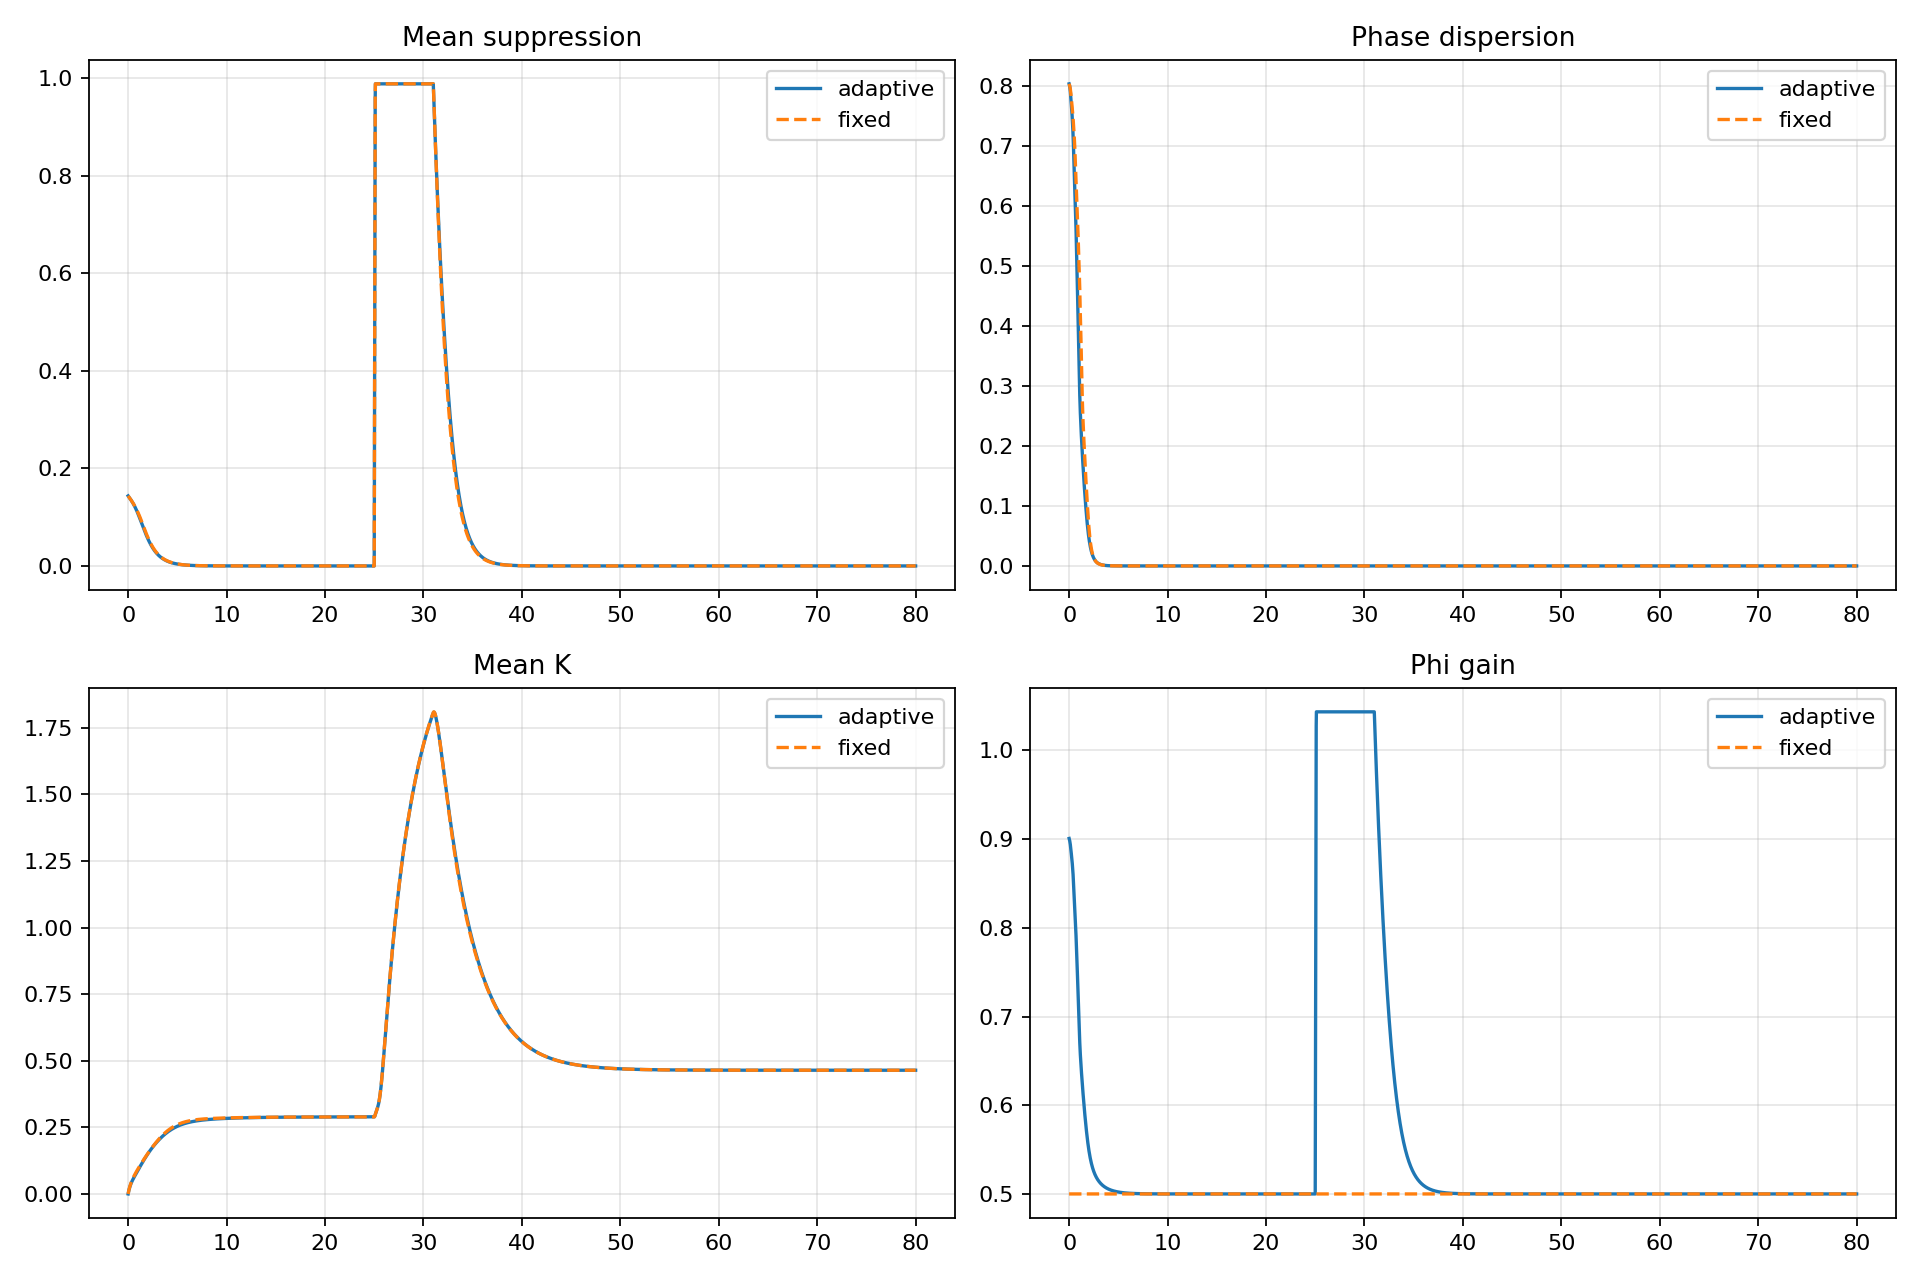
\includegraphics[width=0.85\linewidth]{figures/adaptive_rc_first_demo_plot.png}
    \caption{Initial sanity check for adaptive RC versus fixed RC on a simple stress protocol.}
    \label{fig:vol5_adaptive_sanity}
\end{figure}

\begin{figure}[h]
    \centering
    
\includegraphics[width=0.9\linewidth]{../outputs/attunement_ablation_plot.png}
    \caption{Attunement ablation under repeated lessons. Mutual attunement reduces peak field error even when recovery-time metrics change weakly.}
    \label{fig:vol5_attunement}
\end{figure}

\subsection*{Conclusion Draft}
The main contribution of Volume V is not yet a fully mature learning controller, but a bounded instructor-like coordination framework for heterogeneous networks. The simulations indicate that the most robust current learning effect is mutual attunement between coordinator and group, which reduces field error across repeated lessons even before strong gains appear in coarse recovery-time metrics. This is already a meaningful systems result: adaptive coordination may improve the quality of the field before it improves its speed. At the same time, bounded group memory remains an important secondary extension whose long-horizon role still requires cleaner validation.
